% PressureExpPlatform_3DInsert.tex

\tikzstyle{RectObject}=[rectangle,draw=blue,rounded corners,line width=0.5mm,minimum width=4.0em,%
	minimum height=1em]
\tikzstyle{LabelObject}=[fill=white,rectangle,rounded corners,line width=0.5mm,%
	align=center]
\tikzstyle{ArrowObject}=[red,line width=1.0mm, -latex]

\resizebox{!}{0.45\textwidth}{
  \begin{tikzpicture}
    \node[anchor=south west,inner sep=0] (image) at (0,0)%
		  {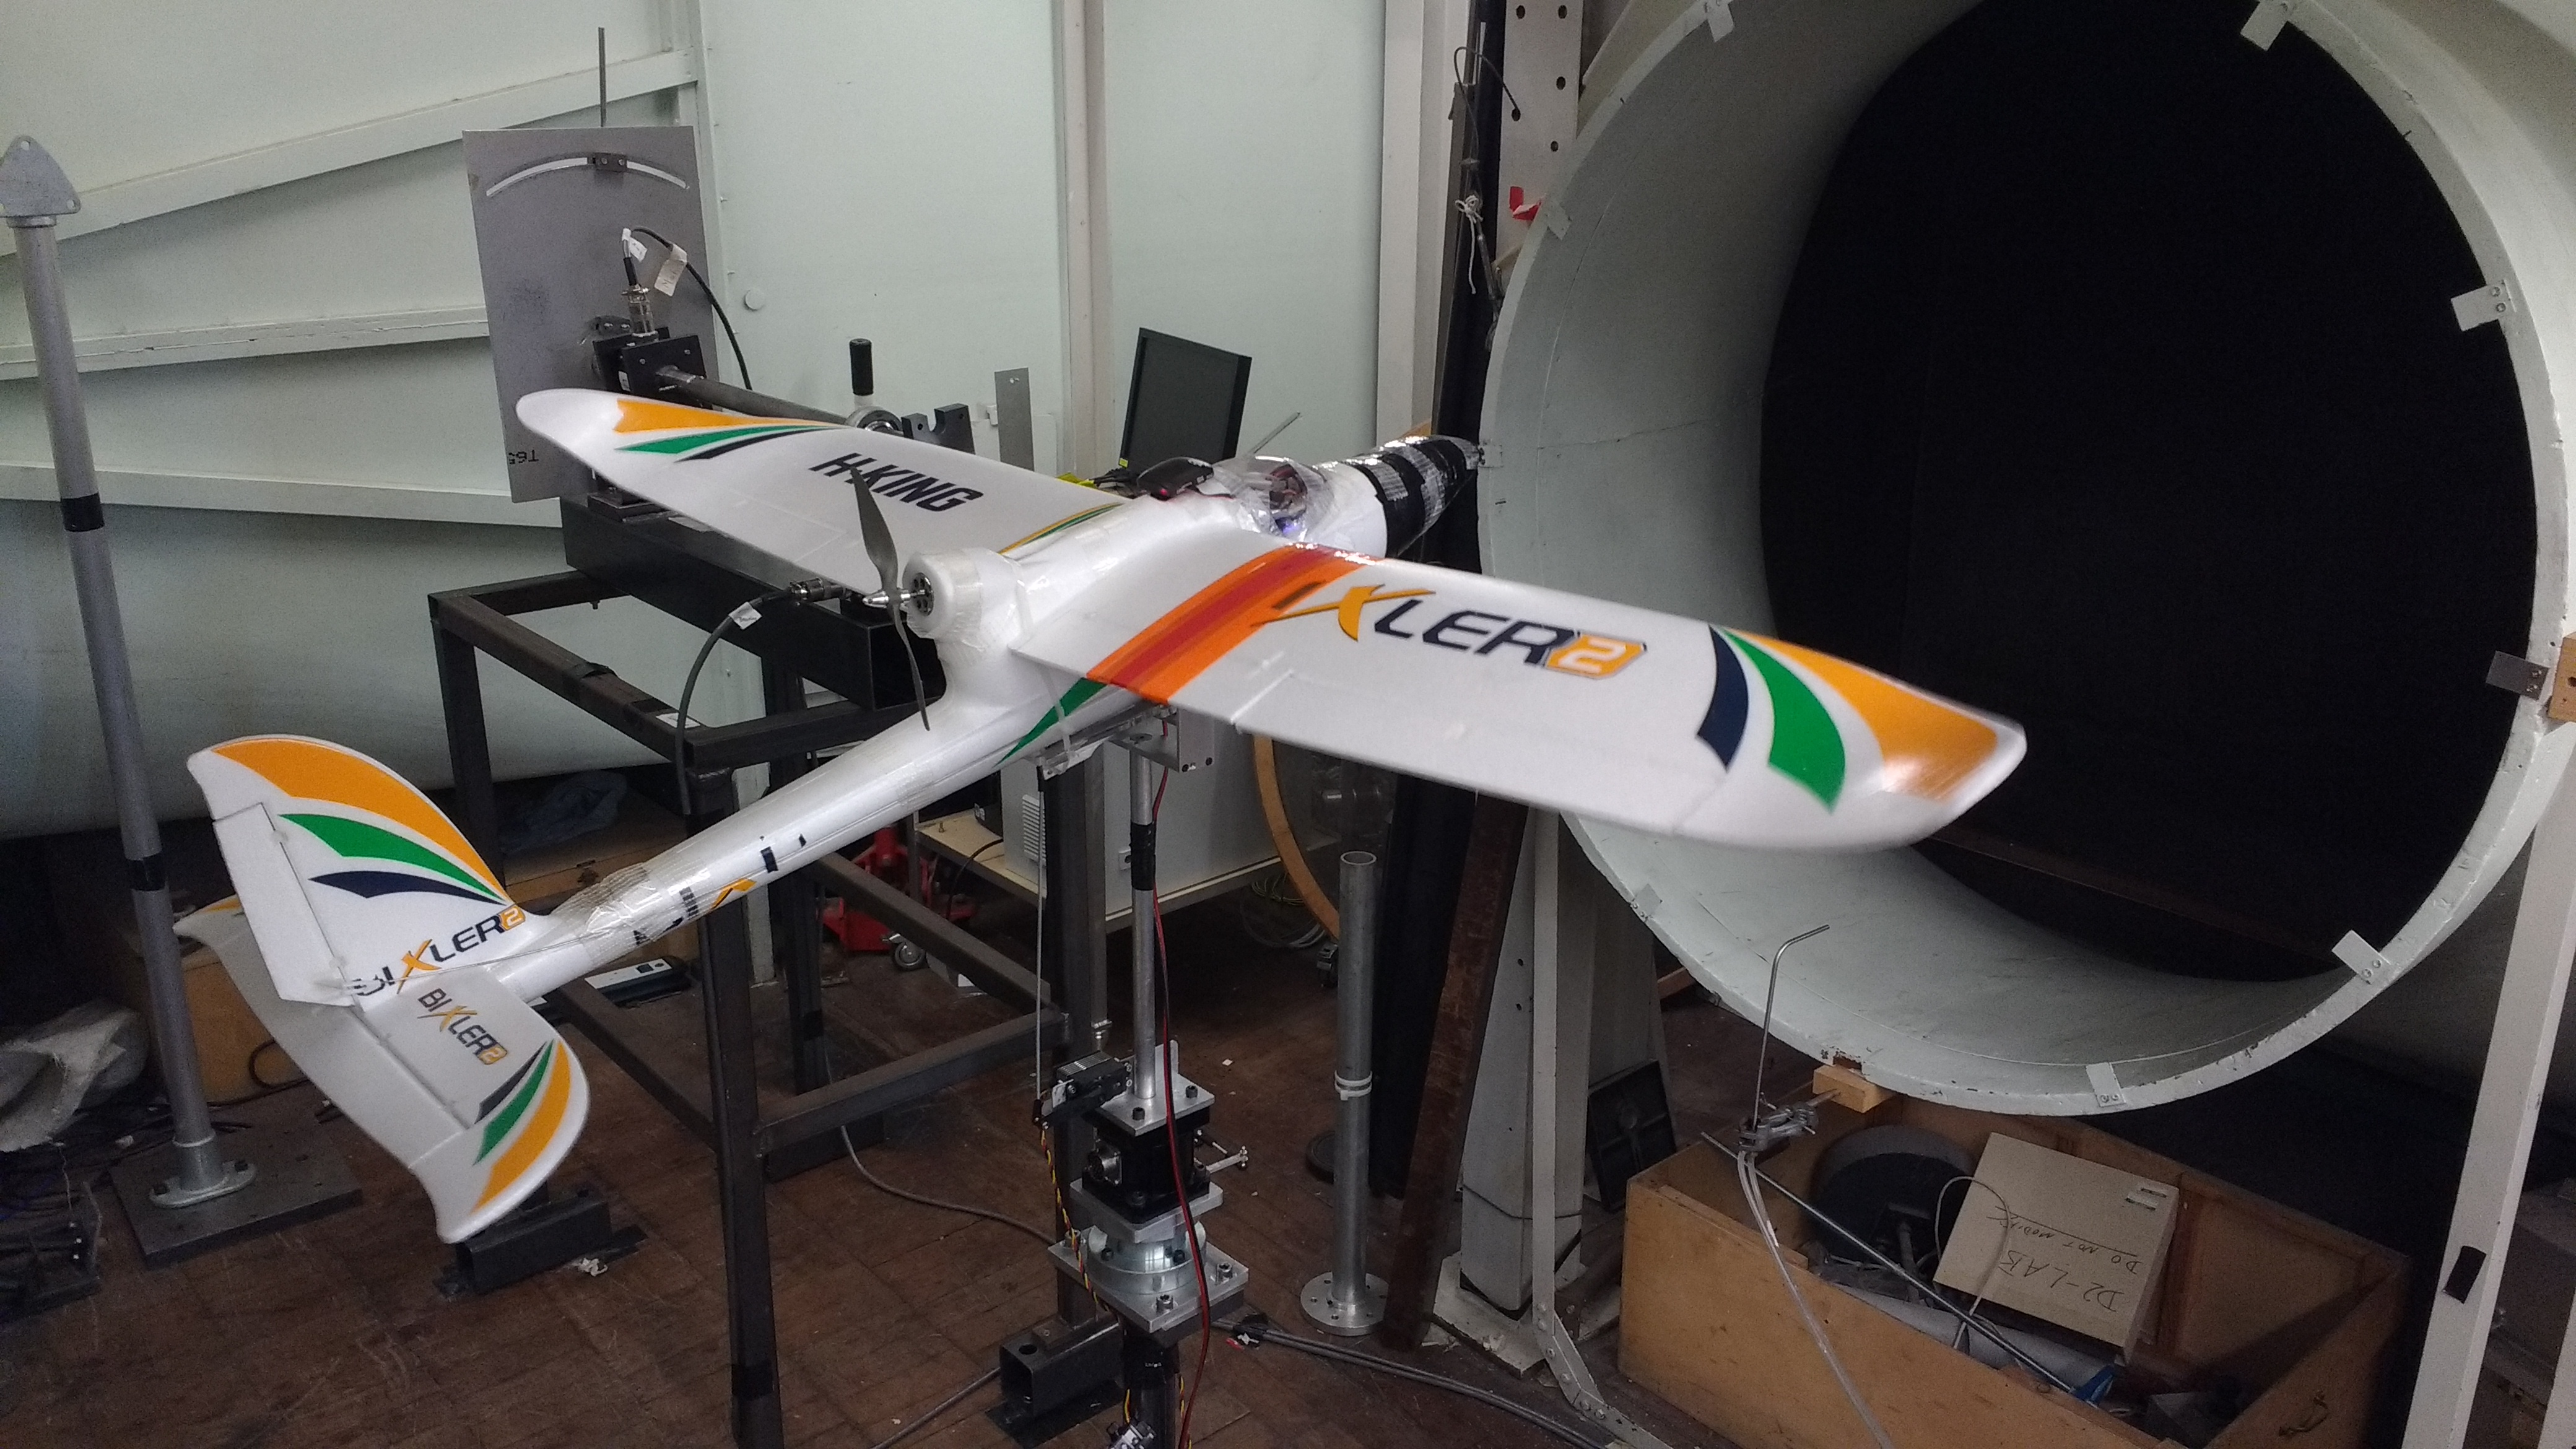
\includegraphics[width=\textwidth]{Bixler_WTTest.eps}};
    % Define scope with 'image' dimensions as reference
    \begin{scope}[x={(image.south east)},y={(image.north west)}]
      %\draw[help lines,xstep=.05,ystep=.05] (0,0) grid (1,1);
      %\foreach \x in {0,1,...,9} { \node [anchor=north] at (\x/10,0) {0.\x}; }
      %\foreach \y in {0,1,...,9} { \node [anchor=east] at (0,\y/10) {0.\y}; }
			
			\only<2>{
			  % Wing 3D printed insert location
			  \draw(0.475,0.575) node[RectObject,rotate around={35:(0,0)}] (WingInsert) {};
			  % Wing 3D printed insert label
			  \draw(0.85,0.85) node[LabelObject] (WingInsert_Label) {3-D Printed\\Insert};
			  % Wing 3D printed insert arrow
			  \draw[ArrowObject] (WingInsert_Label.west) -- (WingInsert.east);
			}
			
    \end{scope}
  \end{tikzpicture}
}